\documentclass{ximera}
\graphicspath{  %% When looking for images,
{./}            %% look here first,
{./pictures/}   %% then look for a pictures folder,
{../pictures/}  %% which may be a directory up.
{../../pictures/}  %% which may be a directory up.
{../../../pictures/}  %% which may be a directory up.
{../../../../pictures/}  %% which may be a directory up.
}

\usepackage{listings}
\usepackage{circuitikz}
\usepackage{xcolor}
\usepackage{amsmath,amsthm}
\usepackage{subcaption}
\usepackage{graphicx}
\usepackage{tikz}
\usepackage{tikz-3dplot}
\usepackage{amsfonts}
\usepackage{mdframed} % For framing content
\usepackage{tikz-cd}

  \renewcommand{\vector}[1]{\left\langle #1\right\rangle}
  \newcommand{\arrowvec}[1]{{\overset{\rightharpoonup}{#1}}}
  \newcommand{\ro}{\texttt{R}}%% row operation
  \newcommand{\dotp}{\bullet}%% dot product
  \renewcommand{\l}{\ell}
  \let\defaultAnswerFormat\answerFormatBoxed
  \usetikzlibrary{calc,bending}
  \tikzset{>=stealth}
  




%make a maroon color
\definecolor{maroon}{RGB}{128,0,0}
%make a dark blue color
\definecolor{darkblue}{RGB}{0,0,139}
%define the color fourier0 to be the maroon color
\definecolor{fourier0}{RGB}{128,0,0}
%define the color fourier1 to be the dark blue color
\definecolor{fourier1}{RGB}{0,0,139}
%define the color fourier 1t to be the light blue color
\definecolor{fourier1t}{RGB}{173,216,230}
%define the color fourier2 to be the dark green color
\definecolor{fourier2}{RGB}{0,100,0}
%define teh color fourier2t to be the light green color
\definecolor{fourier2t}{RGB}{144,238,144}
%define the color fourier3 to be the dark purple color
\definecolor{fourier3}{RGB}{128,0,128}
%define the color fourier3t to be the light purple color
\definecolor{fourier3t}{RGB}{221,160,221}
%define the color fourier0t to be the red color
\definecolor{fourier0t}{RGB}{255,0,0}
%define the color fourier4 to be the orange color
\definecolor{fourier4}{RGB}{255,165,0}
%define the color fourier4t to be the darker orange color
\definecolor{fourier4t}{RGB}{255,215,0}
%define the color fourier5 to be the yellow color
\definecolor{fourier5}{RGB}{255,255,0}
%define the color fourier5t to be the darker yellow color
\definecolor{fourier5t}{RGB}{255,255,100}
%define the color fourier6 to be the green color
\definecolor{fourier6}{RGB}{0,128,0}
%define the color fourier6t to be the darker green color
\definecolor{fourier6t}{RGB}{0,255,0}

%New commands for this doc for errors in copying
\newcommand{\eigenvar}{\lambda}
%\newcommand{\vect}[1]{\mathbf{#1}}
\renewcommand{\th}{^{\text{th}}}
\newcommand{\st}{^{\text{st}}}
\newcommand{\nd}{^{\text{nd}}}
\newcommand{\rd}{^{\text{rd}}}
\newcommand{\paren}[1]{\left(#1\right)}
\newcommand{\abs}[1]{\left|#1\right|}
\newcommand{\R}{\mathbb{R}}
\newcommand{\C}{\mathbb{C}}
\newcommand{\Hilb}{\mathbb{H}}
\newcommand{\qq}[1]{\text{#1}}
\newcommand{\Z}{\mathbb{Z}}
\newcommand{\N}{\mathbb{N}}
\newcommand{\q}[1]{\text{``#1''}}
%\newcommand{\mat}[1]{\begin{bmatrix}#1\end{bmatrix}}
\newcommand{\rref}{\text{reduced row echelon form}}
\newcommand{\ef}{\text{echelon form}}
\newcommand{\ohm}{\Omega}
\newcommand{\volt}{\text{V}}
\newcommand{\amp}{\text{A}}
\newcommand{\Seq}{\textbf{Seq}}
\newcommand{\Poly}{\textbf{P}}
\renewcommand{\quad}{\text{    }}
\newcommand{\roweq}{\simeq}
\newcommand{\rowop}{\simeq}
\newcommand{\rowswap}{\leftrightarrow}
\newcommand{\Mat}{\textbf{M}}
\newcommand{\Func}{\textbf{Func}}
\newcommand{\Hw}{\textbf{Hamming weight}}
\newcommand{\Hd}{\textbf{Hamming distance}}
\newcommand{\rank}{\text{rank}}
\newcommand{\longvect}[1]{\overrightarrow{#1}}
% Define the circled command
\newcommand{\circled}[1]{%
  \tikz[baseline=(char.base)]{
    \node[shape=circle,draw,inner sep=2pt,red,fill=red!20,text=black] (char) {#1};}%
}

% Define custom command \strikeh that just puts red text on the 2nd argument
\newcommand{\strikeh}[2]{\textcolor{red}{#2}}

% Define custom command \strikev that just puts red text on the 2nd argument
\newcommand{\strikev}[2]{\textcolor{red}{#2}}

%more new commands for this doc for errors in copying
\newcommand{\SI}{\text{SI}}
\newcommand{\kg}{\text{kg}}
\newcommand{\m}{\text{m}}
\newcommand{\s}{\text{s}}
\newcommand{\norm}[1]{\left\|#1\right\|}
\newcommand{\col}{\text{col}}
\newcommand{\sspan}{\text{span}}
\newcommand{\proj}{\text{proj}}
\newcommand{\set}[1]{\left\{#1\right\}}
\newcommand{\degC}{^\circ\text{C}}
\newcommand{\centroid}[1]{\overline{#1}}
\newcommand{\dotprod}{\boldsymbol{\cdot}}
%\newcommand{\coord}[1]{\begin{bmatrix}#1\end{bmatrix}}
\newcommand{\iprod}[1]{\langle #1 \rangle}
\newcommand{\adjoint}{^{*}}
\newcommand{\conjugate}[1]{\overline{#1}}
\newcommand{\eigenvarA}{\lambda}
\newcommand{\eigenvarB}{\mu}
\newcommand{\orth}{\perp}
\newcommand{\bigbracket}[1]{\left[#1\right]}
\newcommand{\textiff}{\text{ if and only if }}
\newcommand{\adj}{\text{adj}}
\newcommand{\ijth}{\emph{ij}^\text{th}}
\newcommand{\minor}[2]{M_{#2}}
\newcommand{\cofactor}{\text{C}}
\newcommand{\shift}{\textbf{shift}}
\newcommand{\startmat}[1]{
  \left[\begin{array}{#1}
}
\newcommand{\stopmat}{\end{array}\right]}
%a command to give a name to explorations and hints and theorems
\newcommand{\name}[1]{\begin{centering}\textbf{#1}\end{centering}}
\newcommand{\vect}[1]{\vec{#1}}
\newcommand{\dfn}[1]{\textbf{#1}}
\newcommand{\transpose}{\mathsf{T}}
\newcommand{\mtlb}[2][black]{\texttt{\textcolor{#1}{#2}}}
\newcommand{\RR}{\mathbb{R}} % Real numbers
\newcommand{\id}{\text{id}}

\author{Zack Reed}
%borrowed from selinger linear algebra
\begin{document}

\section*{Exercises}

\begin{exercise}
  Consider $\R^3$ with the usual dot product. Let
  \begin{equation*}
    \vect{u}_1 = \startmat{r} -1 \\ 1 \\ 1 \stopmat,
    \quad
    \vect{u}_2 = \startmat{r} -1 \\ -2 \\ 1 \stopmat,
    \quad\mbox{and}\quad
    \vect{v} = \startmat{r} -1 \\ 5 \\ 3 \stopmat.
  \end{equation*}
  Note that $\vect{u}_1$ and $\vect{u}_2$ are orthogonal.
  Find the best approximation of $\vect{v}$ in $\sspan\set{\vect{u}_1,
    \vect{u}_2}$.
  \begin{solution}
    The best approximation is $\vect{v}' = 3\vect{u}_1 - \vect{u}_2 =
    \startmat{r} -2 \\ 5 \\ 2 \stopmat$.
  \end{solution}
\end{exercise}

\begin{exercise}
  Consider $\R^4$ with the usual dot product. Let
  \begin{equation*}
    \vect{u}_1 = \startmat{r} 0 \\ 0 \\ 1 \\ 3 \stopmat,
    \quad
    \vect{u}_2 = \startmat{r} 1 \\ 1 \\ 0 \\ 0 \stopmat,
    \quad
    \vect{u}_3 = \startmat{r} 1 \\ -1 \\ 3 \\ -1 \stopmat,
    \quad\mbox{and}\quad
    \vect{v} = \startmat{r} 6 \\  -2 \\ -5 \\  5 \stopmat.
  \end{equation*}
  Note that $\vect{u}_1$, $\vect{u}_2$, and $\vect{u}_3$ are
  orthogonal.  Find the best approximation of $\vect{v}$ in
  $\sspan\set{\vect{u}_1,\vect{u}_2, \vect{u}_3}$.
  \begin{solution}
    The best approximation is
    $\vect{v}' = \vect{u}_1 + 2\vect{u}_2 - \vect{u}_3
    = \startmat{r} 1 \\ 3 \\ -2 \\ 4 \stopmat$.
  \end{solution}
\end{exercise}

\begin{exercise}
  In the inner product space $V=C[-1,1]$, consider the function
  $f\in V$ given by
  \begin{equation*}
    f(x)
    ~=~ \begin{cases}
      1 & \text{if $x<0$,} \\
      1-x & \text{if $x\geq 0$.}
    \end{cases}
  \end{equation*}
  Find the closest approximation to $f$ by a polynomial of degree at
  most 0, 1, 2, 3, and 4. Graph both $f$ and the approximating
  polynomials.
  \begin{solution}
    Let $p_0,p_1,\ldots$ be the Legendre polynomials from Section~\ref{sec:gram-schmidt}.
    The approximating polynomials are:
    \begin{eqnarray*}
      f_0(x) &=& \frac{3}{4}p_0, \\
      f_1(x) &=& \frac{3}{4}p_0 - \frac{1}{2}p_1, \\
      f_2(x) &=& \frac{3}{4}p_0 - \frac{1}{2}p_1 - \frac{15}{32}p_2, \\
      f_3(x) &=& \frac{3}{4}p_0 - \frac{1}{2}p_1 - \frac{15}{32}p_2 + 0p_3, \\
      f_4(x) &=& \frac{3}{4}p_0 - \frac{1}{2}p_1 - \frac{15}{32}p_2 + 0p_3 + \frac{105}{256}p_4.
    \end{eqnarray*}
    \begin{center}
      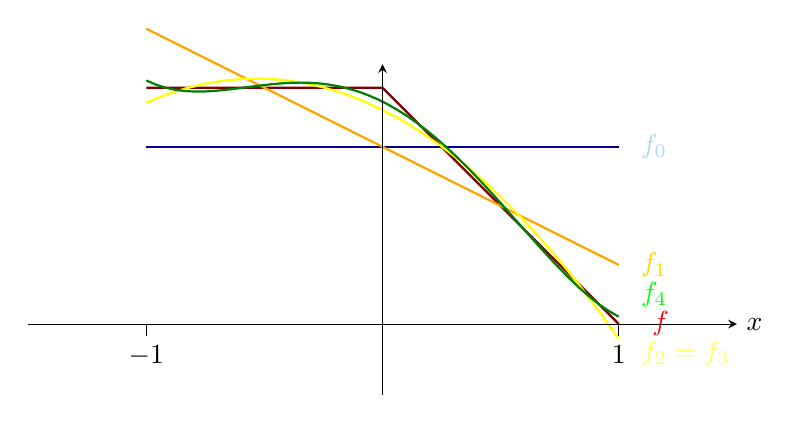
\begin{tikzpicture}[domain=-1:1, scale=3, samples=25]
        \def\fA#1{1}
        \def\fB#1{(#1)}
        \def\fC#1{(abs((#1)^2)-1/3)}
        \def\fD#1{((#1)^3-3/5*(#1))}
        \def\fE#1{(abs((#1)^4)-6/7*abs((#1)^2)+3/35)}
        \def\fF#1{((#1)^5 - 10/9*(#1)^3+5/21*(#1))}
        \def\fG#1{(abs((#1)^6)-15/11*abs((#1)^4)+5/11*abs((#1)^2)-5/231)}
        \def\fH#1{((429*(#1)^7 - 693*(#1)^5 + 315*(#1)^3 - 35*(#1))/429)}
        \def\fI#1{((6435*abs((#1)^8)-12012*abs((#1)^6)+6930*abs((#1)^4)-1260*abs((#1)^2)+35)/6435)}
        \draw[thick,color=fourier0] (-1,1) -- (0,1) -- (1,0);
        \path[color=fourier0t] (1,0) node[right=2ex] {$f$};
        \draw[thick,color=fourier1]         plot (\x,{0.75*\fA{\x}}) (1,0.75) node[right=1ex,color=fourier1t] {$f_0$};
        \draw[thick,color=fourier4]          plot (\x,{0.75*\fA{\x} - 0.5*\fB{\x}}) (1,0.25) node[right=1ex,color=fourier4t] {$f_1$};
        \draw[thick,color=fourier5]      plot (\x,{0.75*\fA{\x} - 0.5*\fB{\x} - 15/32*\fC{\x}}) (1,-0.125) node[right=1ex,color=fourier5t] {$f_2=f_3$};
        \draw[thick,color=fourier6,samples=50] plot (\x,{0.75*\fA{\x} - 0.5*\fB{\x} - 15/32*\fC{\x} + 105/256*\fE{\x}}) (1,0.125) node[right=1ex,fourier6t] {$f_4$};
        \draw[->] (-1.5,0) -- (1.5,0) node[right] {$x$};
        \draw[->] (0,-0.3) -- (0,1.1);
        \draw (1,0) -- (1,-0.05) node[below] {$1$};
        \draw (-1,0) -- (-1,-0.05) node[below] {$-1$};
      \end{tikzpicture}
    \end{center}
  \end{solution}
\end{exercise}

\begin{exercise}
  In the inner product space $C[-\pi,\pi]$, consider the orthogonal
  set of functions from Example~\ref{exa:orthogonal-set-sin-cos}:
  $\set{1, \sin x, \cos x, \sin 2x, \cos 2x, \sin 3x, \cos 3x, \ldots}$.  Let
  $f(x) = x^2$, where $x\in[-\pi,\pi]$. Find the Fourier series of
  $f$.
  \begin{solution}
    $\frac{\pi^2}{3} - \frac{4}{1}\cos x + \frac{4}{4}\cos 2x - \frac{4}{9} \cos 3x + \frac{4}{16} \cos 4x - \frac{4}{25} \cos 5x \pm \ldots$.
  \end{solution}
\end{exercise}


\end{document}